% Activate the following line by filling in the right side. If for example the name of the root file is Main.tex, write
% "...root = Main.tex" if the chapter file is in the same directory, and "...root = ../Main.tex" if the chapter is in a subdirectory.
 
% !TEX root = ../thesis.tex 

\begin{appendices}
\addtocontents{toc}{\protect\setcounter{tocdepth}{0}}
\chapter{Data use statement}

Data was provided by the Human Connectome Project, WU-Minn Consortium (Principal Investigators: David Van Essen and Kamil Ugurbil; 1U54MH091657) funded by the 16 NIH Institutes and Centers that support the NIH Blueprint for Neuroscience Research; and by the McDonnell Center for Systems Neuroscience at Washington University.


\addtocontents{toc}{\protect\setcounter{tocdepth}{1}}
  \chapter{Appendix to chapter \ref{tob_pv_chapter}}
  \section{Evaluation of surface-based PV estimation methods}
The following figures contain the results from all comparator methods for the evaluation of surface-based PV estimation performed in section \ref{tob_pv_evaluation}. 

\begin{figure}
\centering
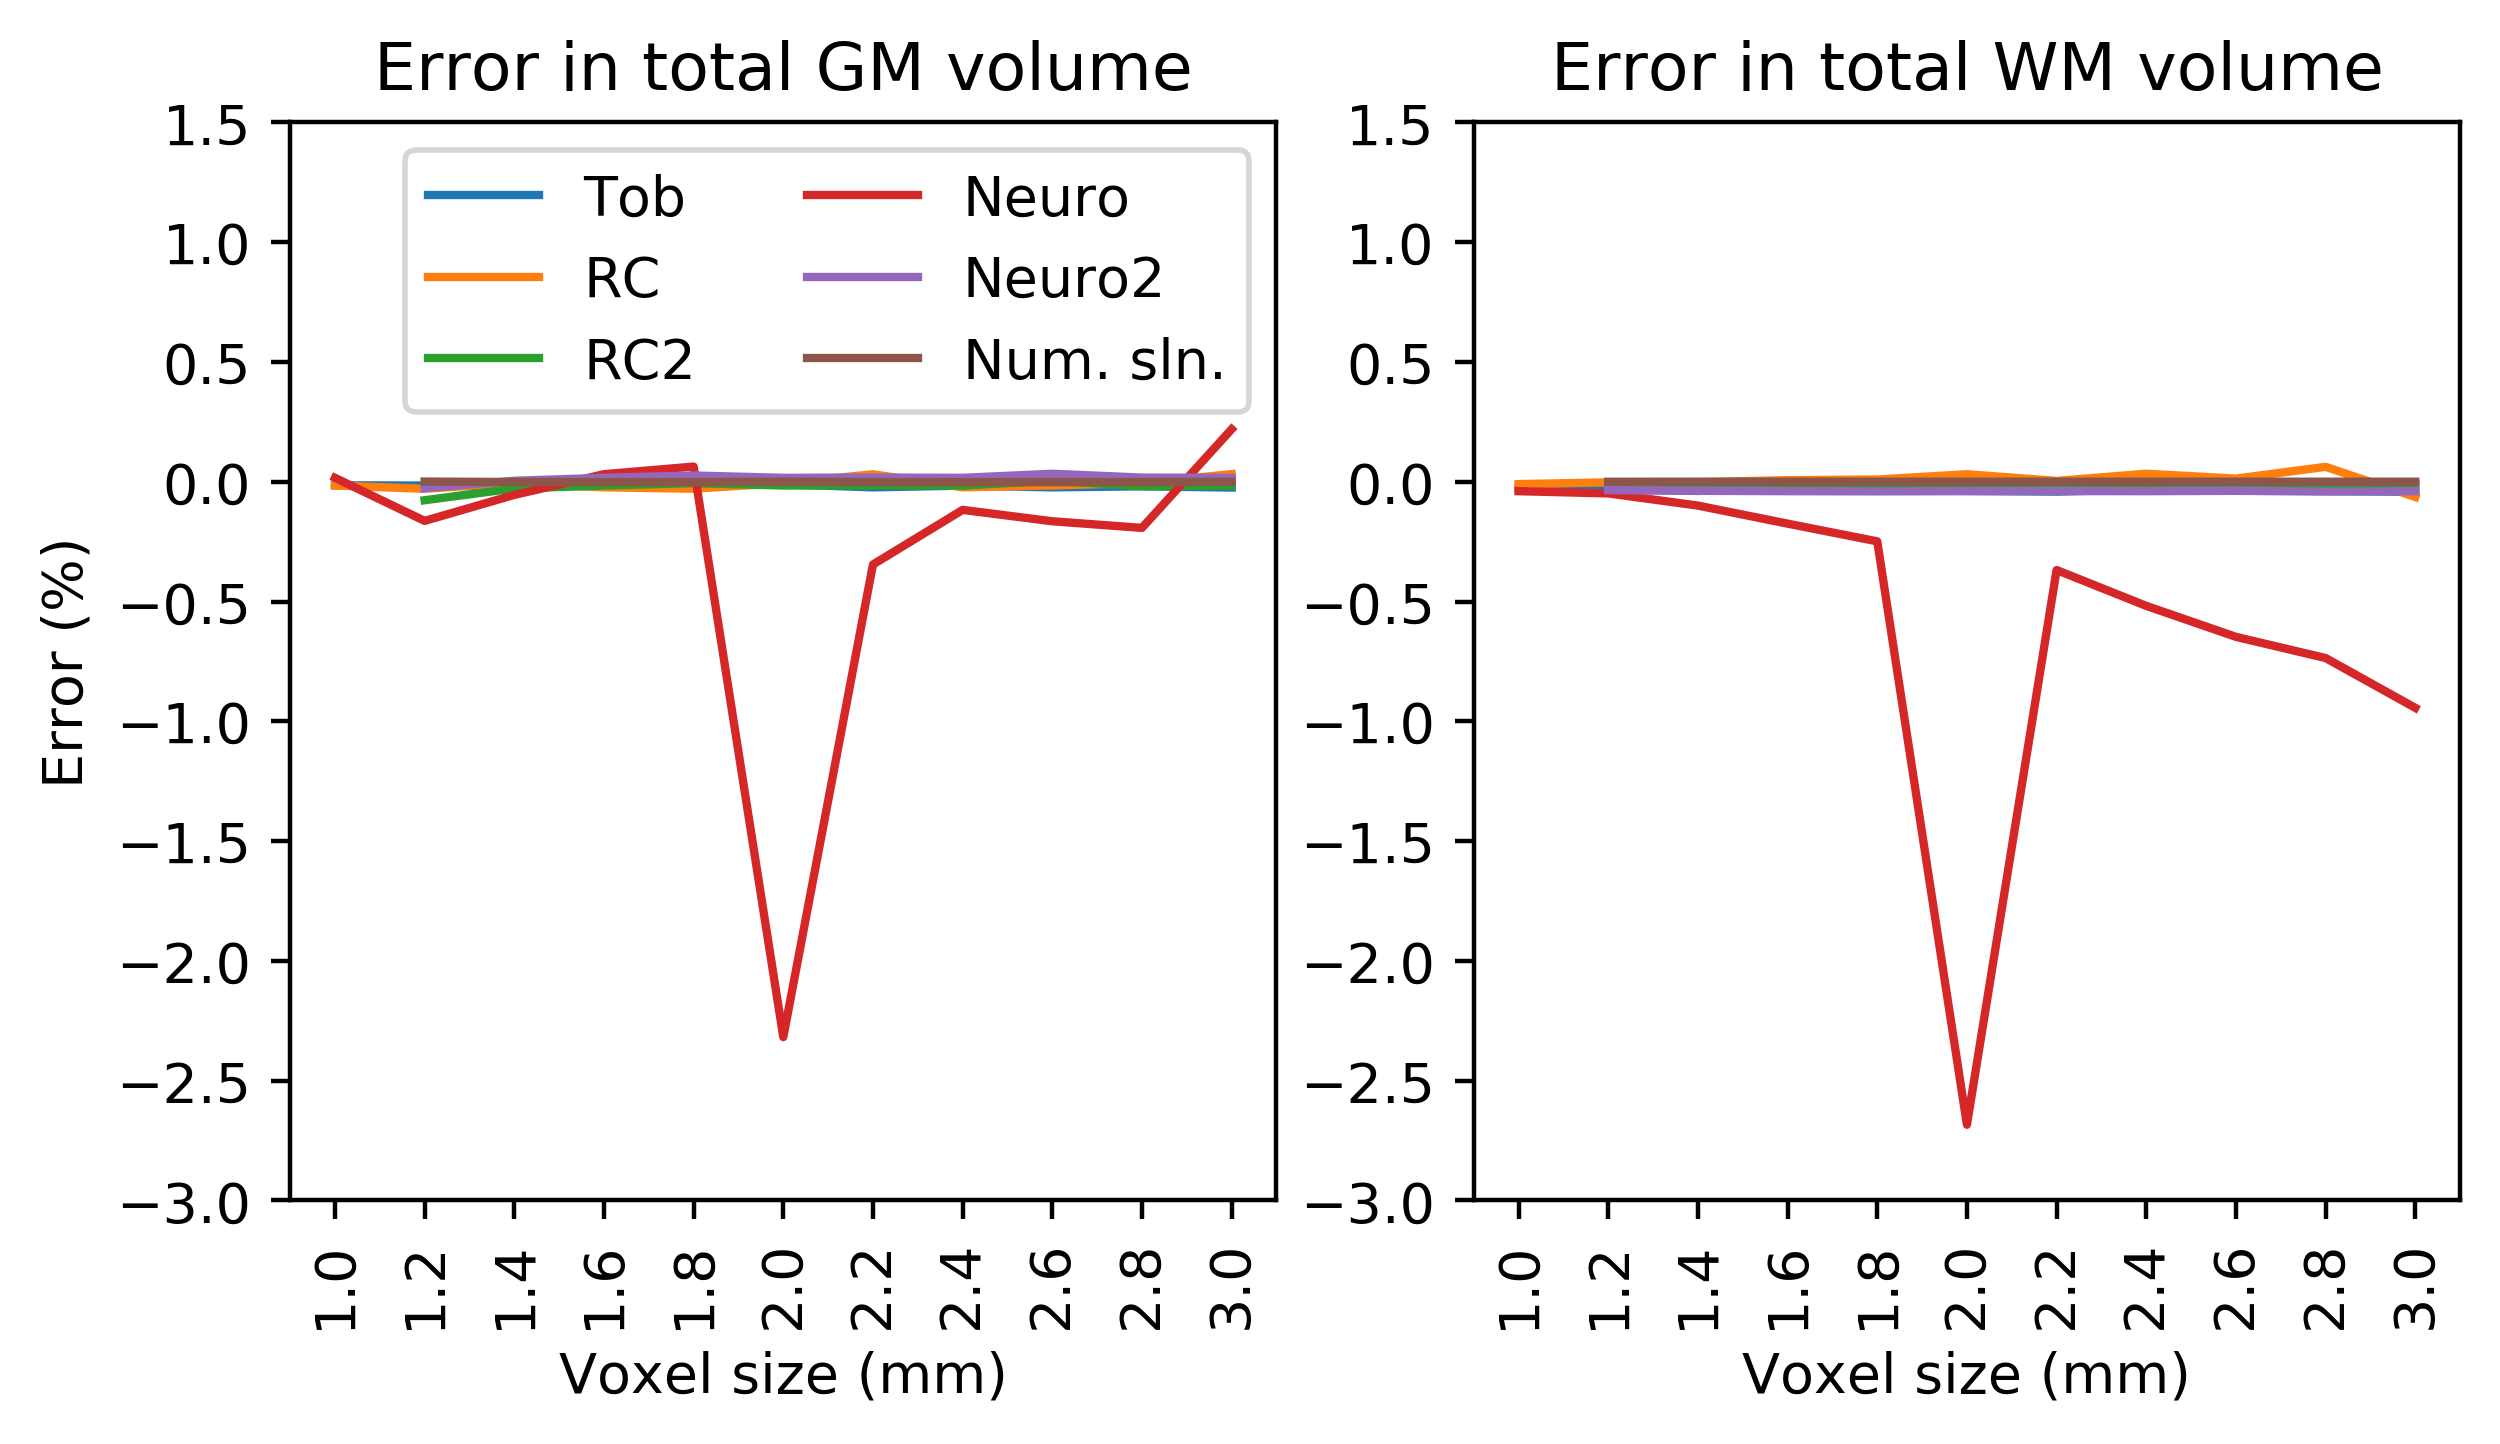
\includegraphics[width = 0.8\textwidth]{tob_sim_total_supp.png}
\caption{Simulated surfaces: error in total tissue volume, all methods. The notch in the Neuro method at 2mm is thought to arise due to an interplay between the number of expanded surfaces created (five) and the voxel size. }
\label{tob_sim_total_supp}
\end{figure}

\begin{figure}
\centering
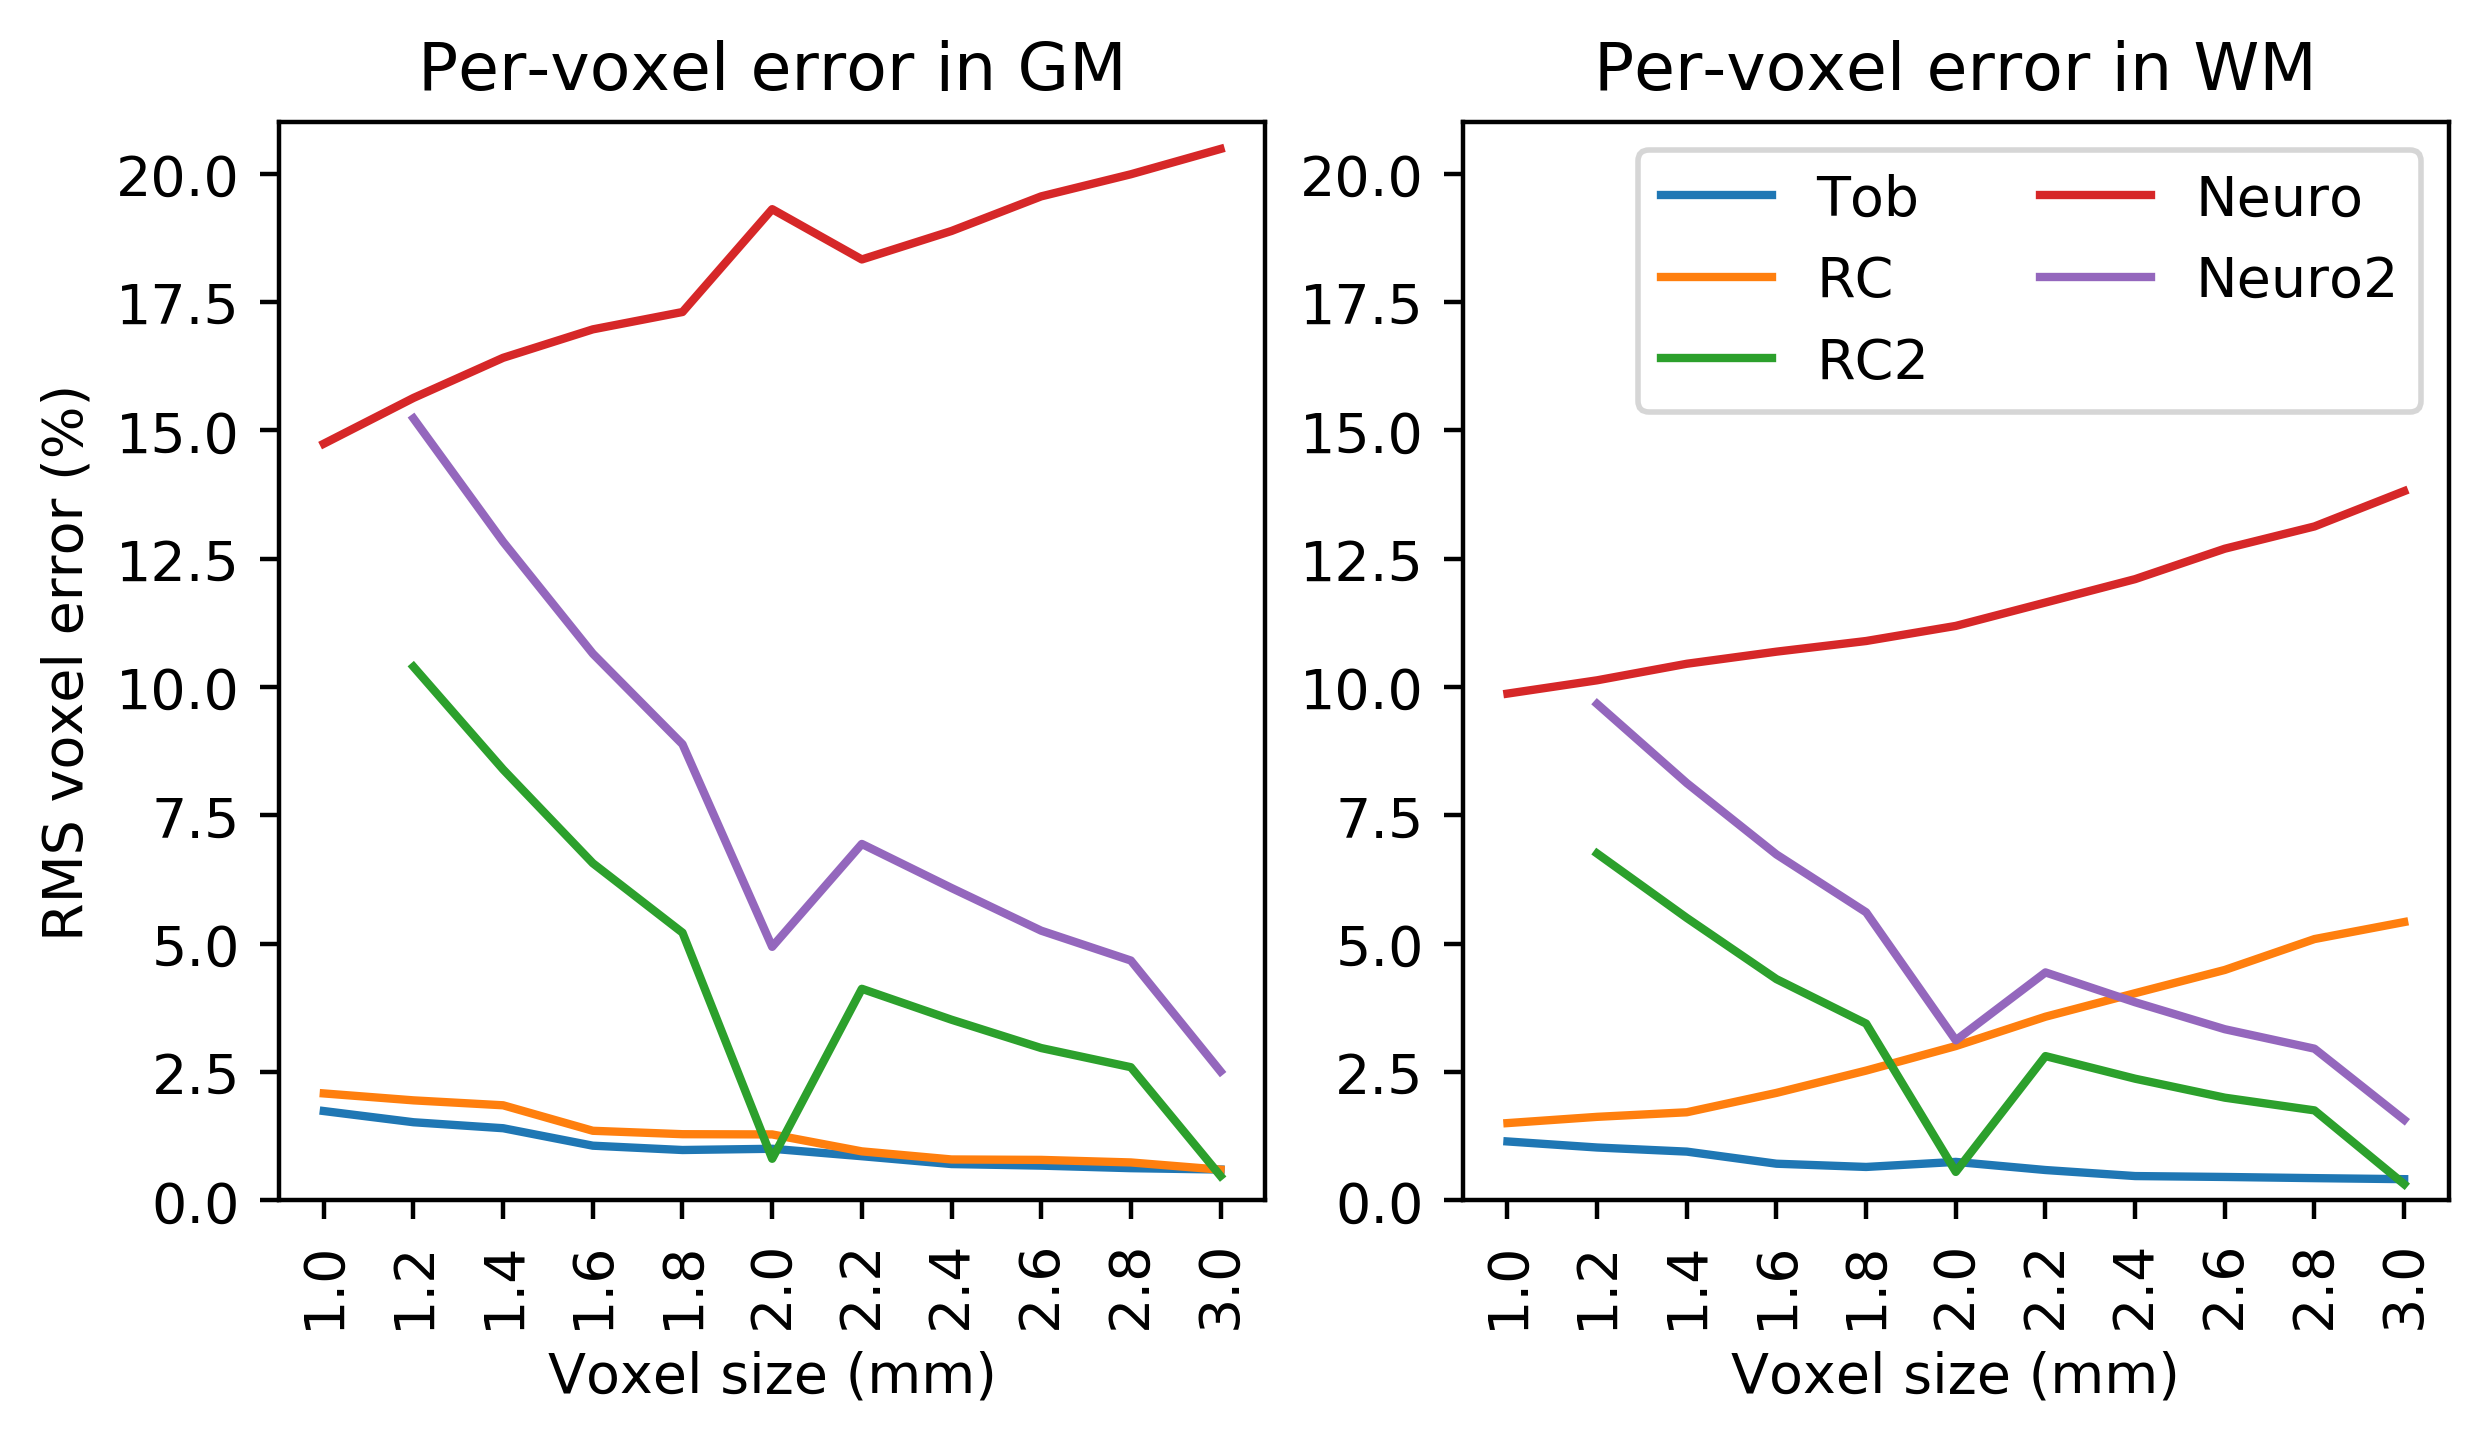
\includegraphics[width = 0.8\textwidth]{tob_sim_voxel_supp.png}
\caption{Simulated surfaces: RMS per-voxel error. Neuro’s results were significantly worse than all other methods at all other resolutions, though the resampled version (Neuro2) performed better. }
\label{tob_sim_voxel_supp}
\end{figure}

\begin{figure}
\centering
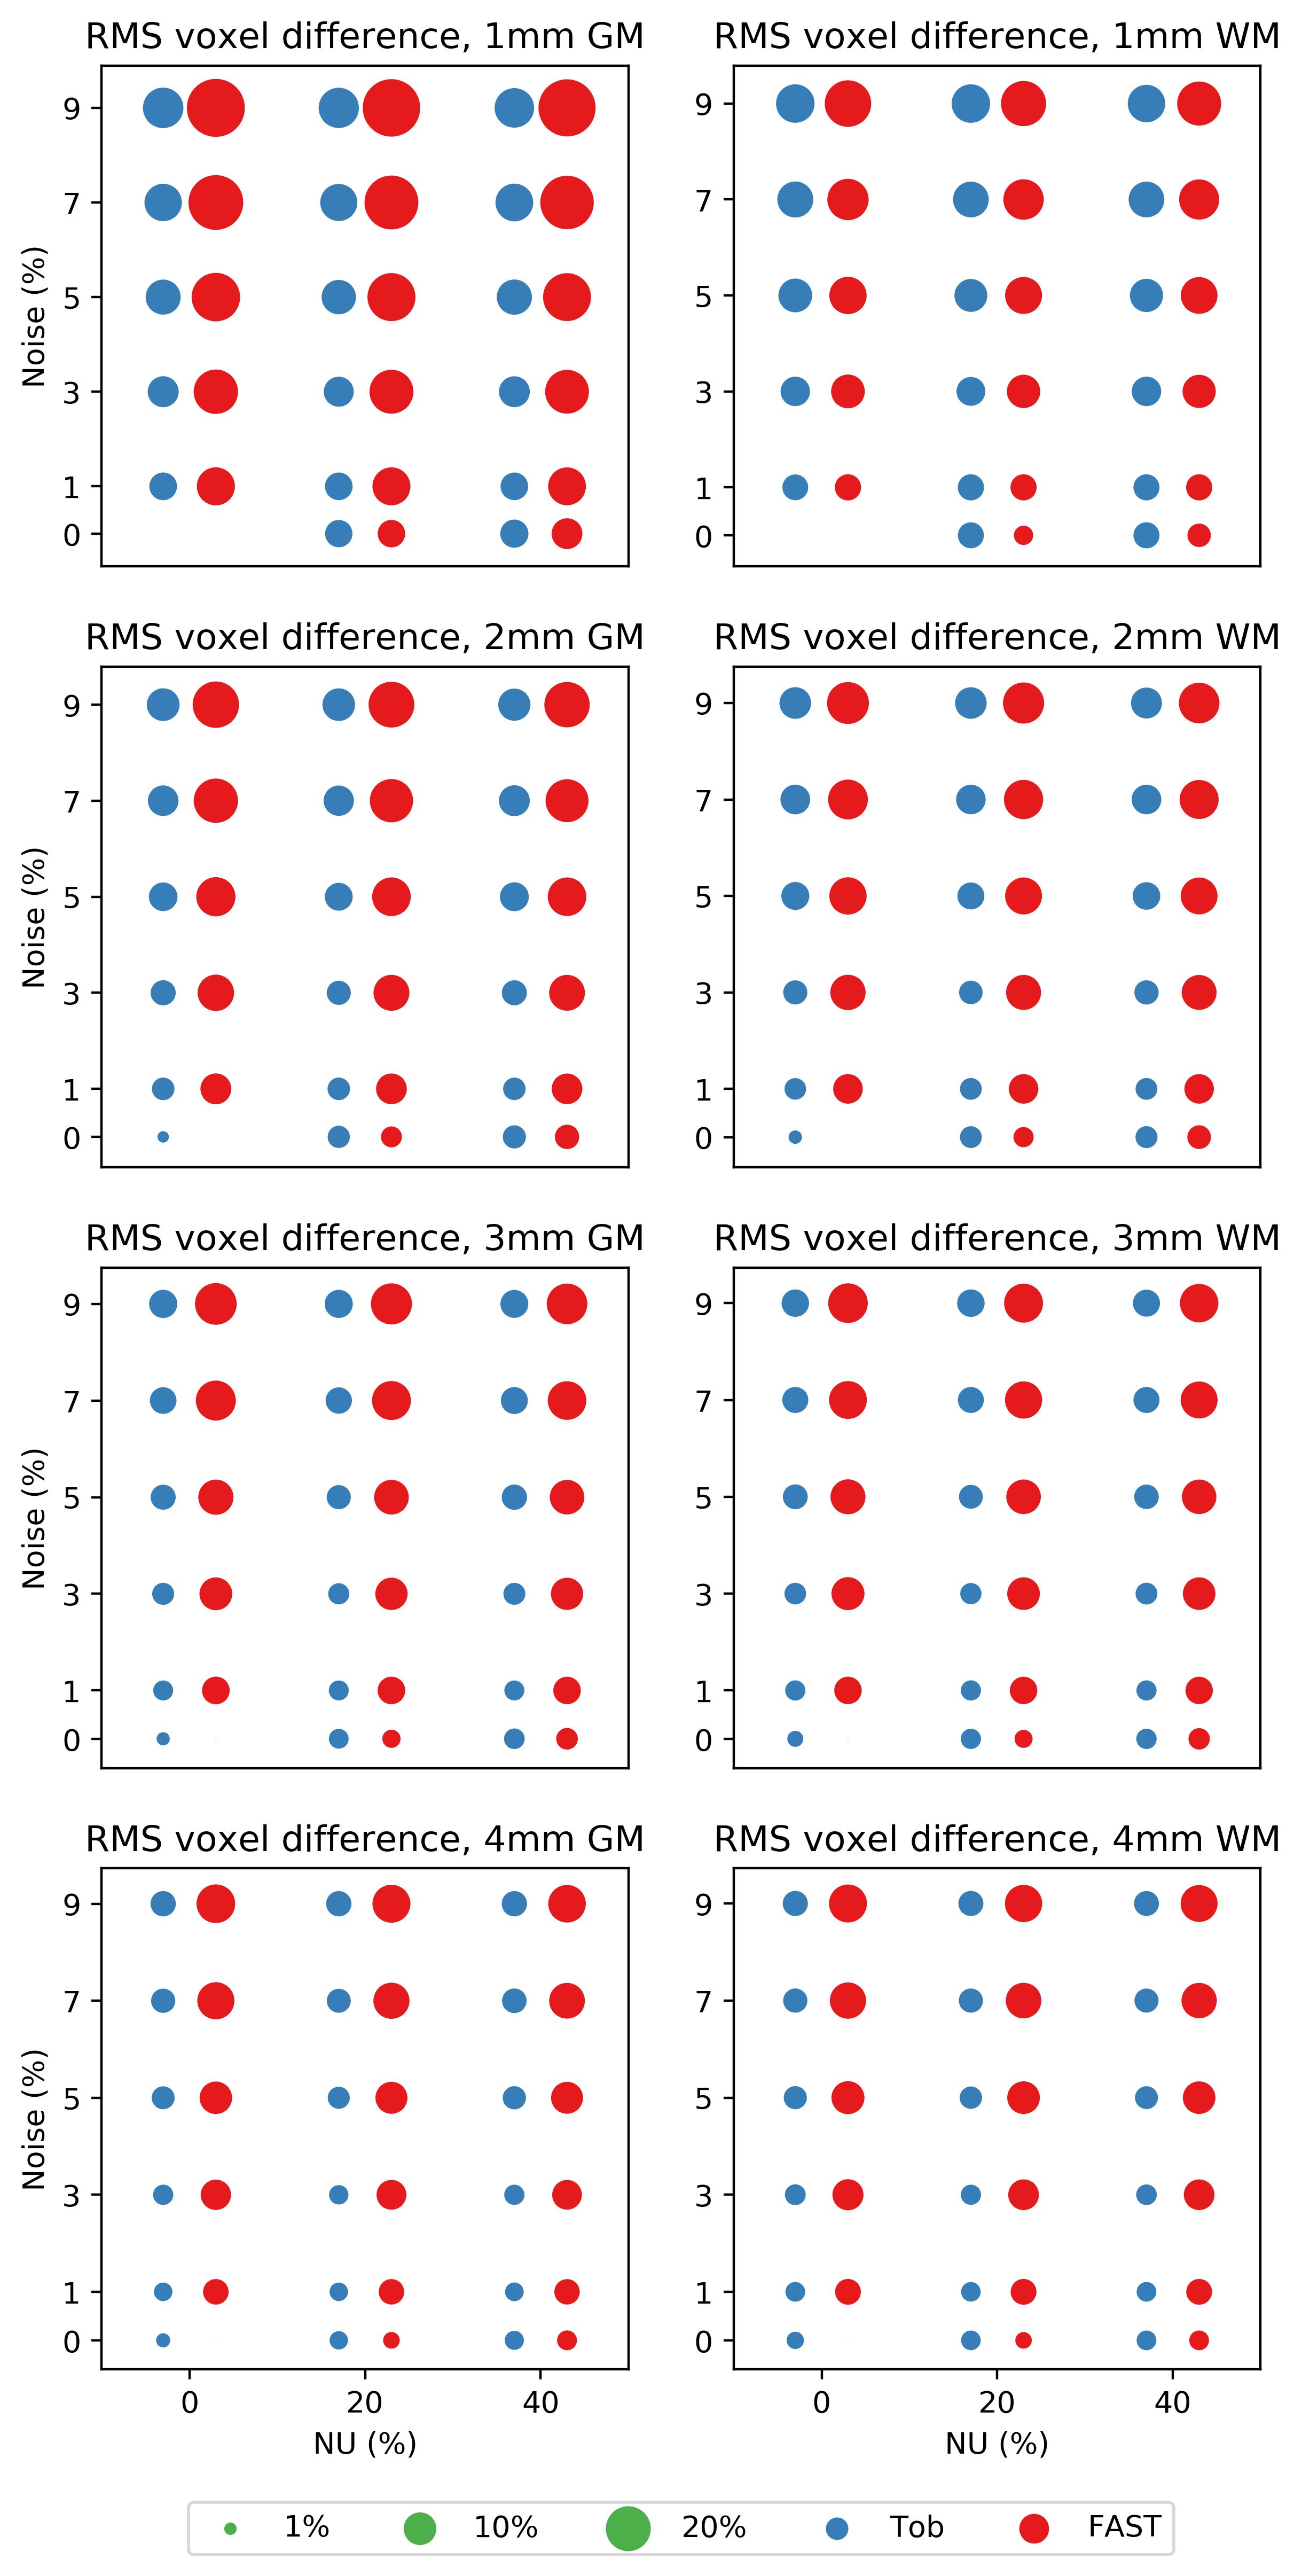
\includegraphics[width = 0.65\textwidth]{brainweb_voxel_supp.png}
\caption{BrainWeb: RMS per-voxel differences at voxel sizes of 1 to 4mm isotropic, referenced to each method’s 1mm 0\% noise 0\% NU results. Toblerone’s differences were smaller at almost all levels of noise and NU, the exception being 0\% noise.  }
\label{brainweb_voxel_supp}
\end{figure}

\begin{figure}
\centering
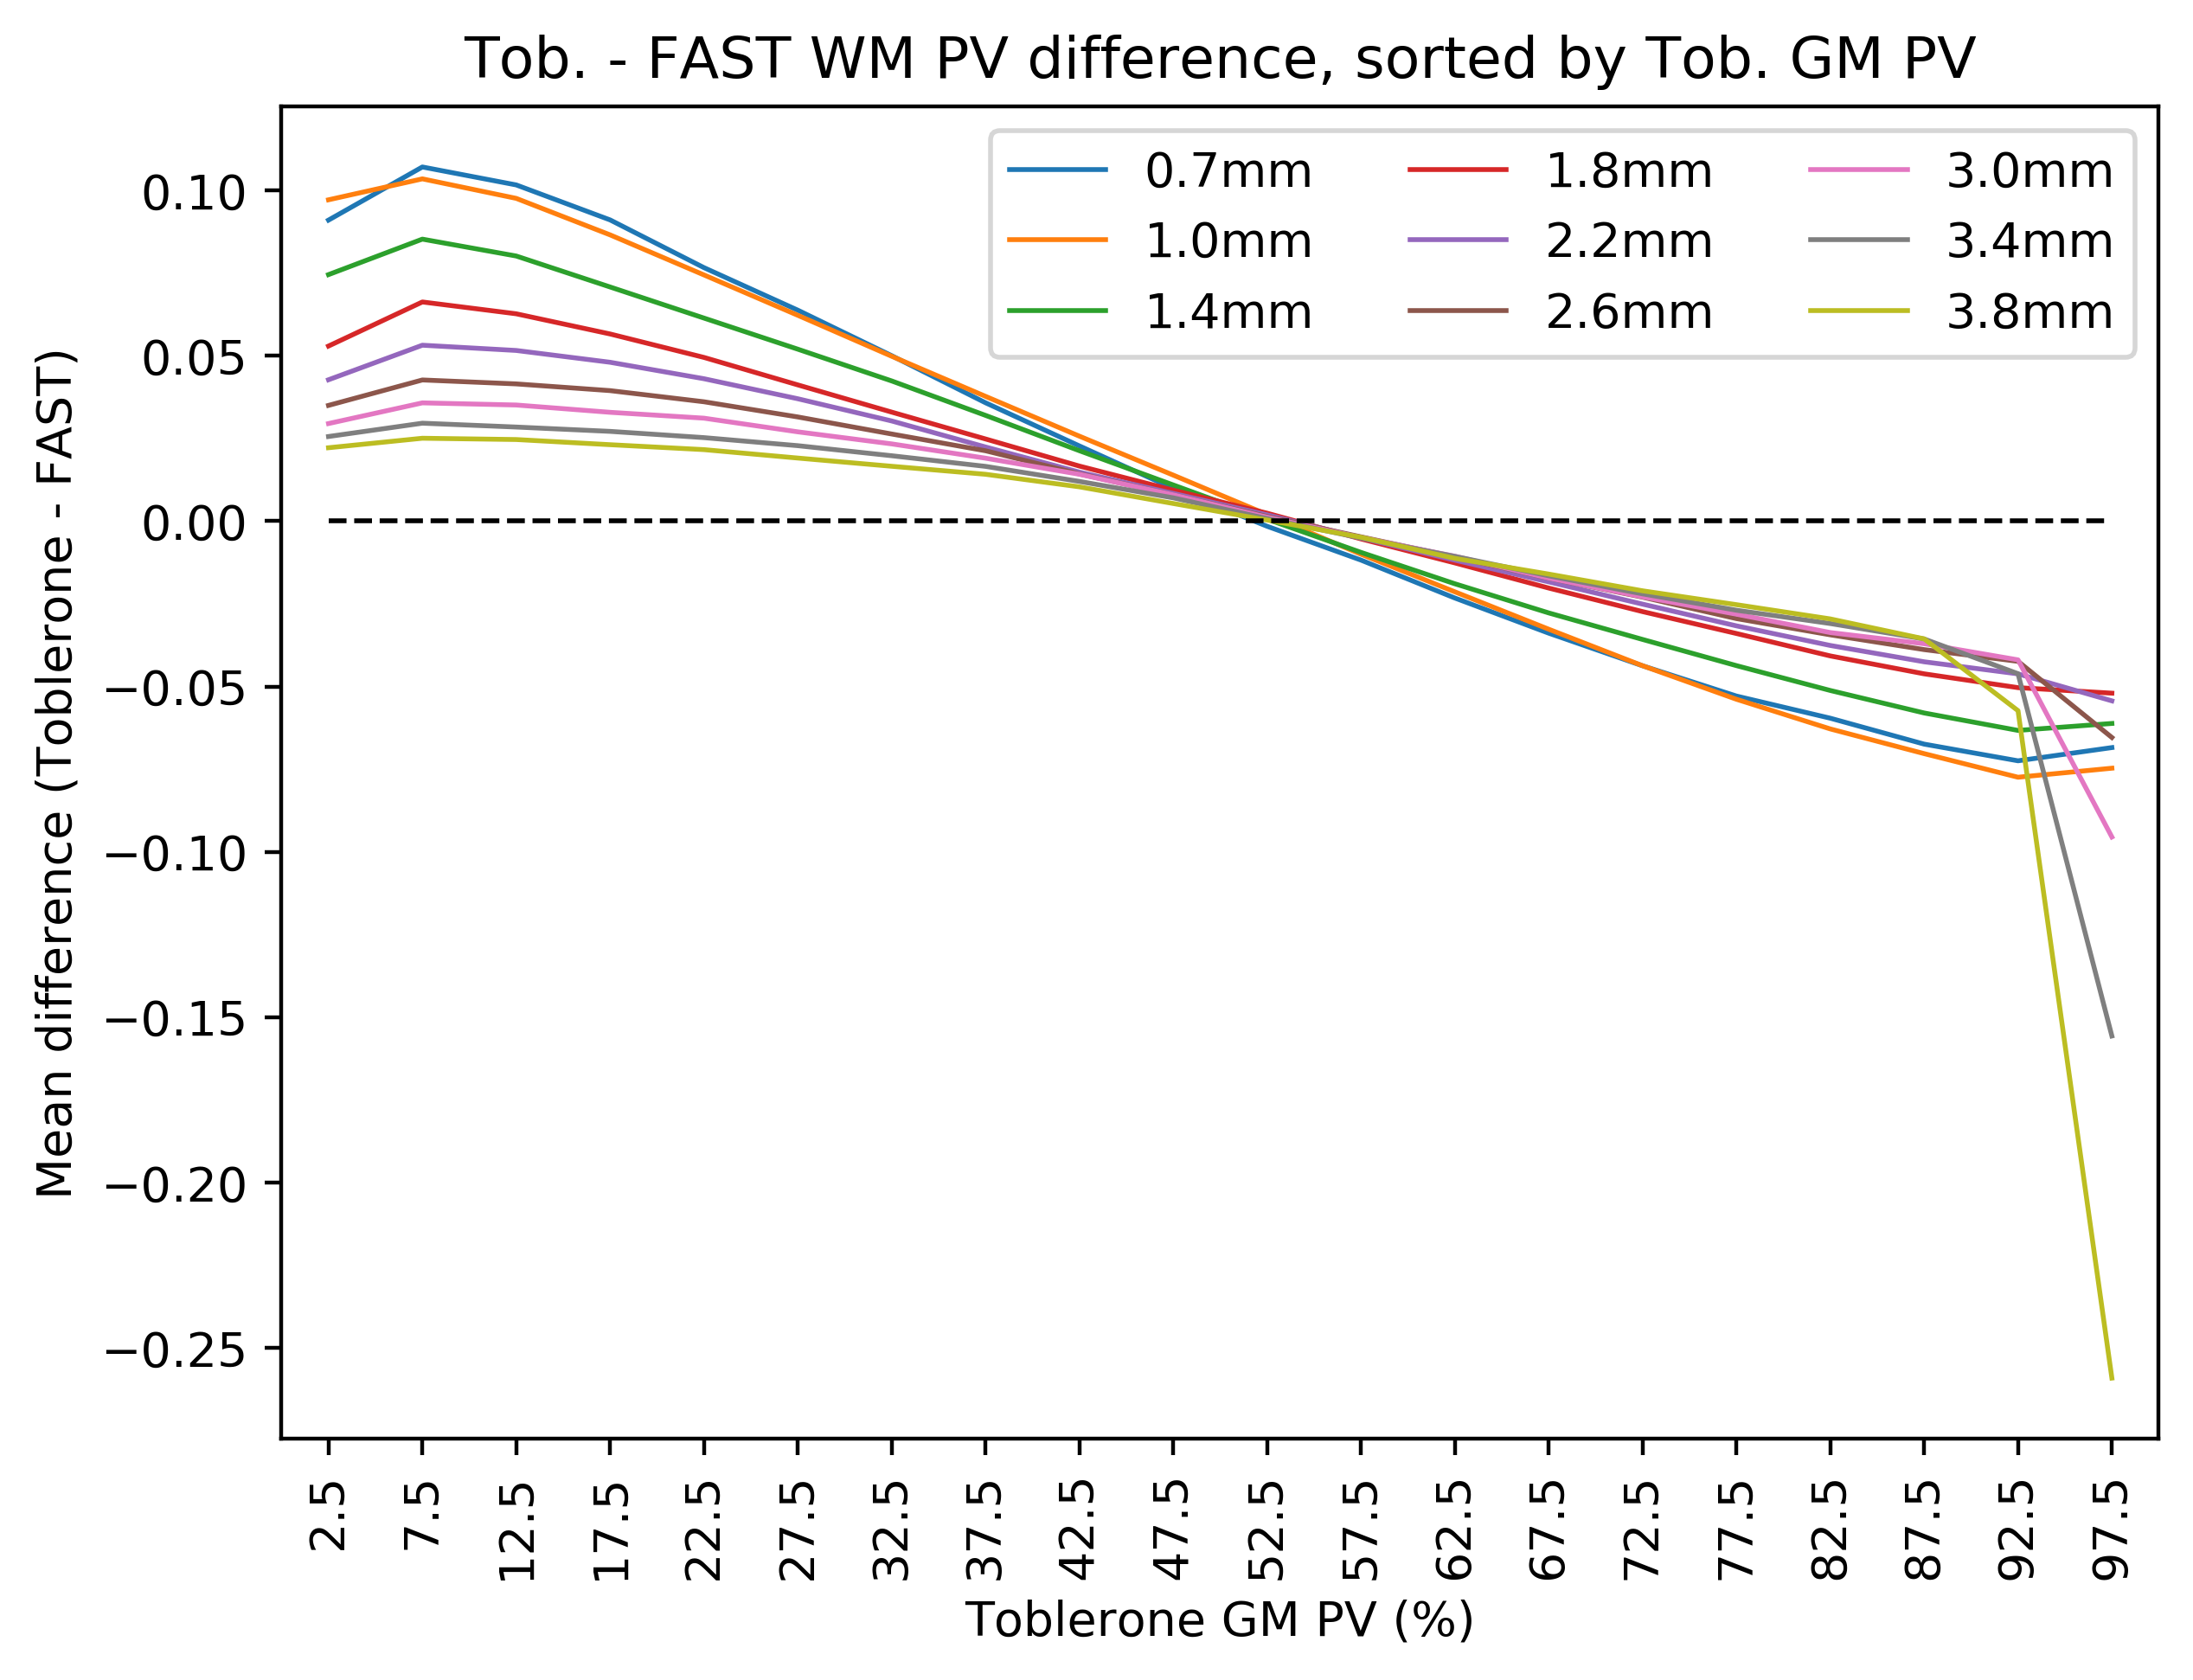
\includegraphics[width = 0.7\textwidth]{hcp_difference_wm_supp.png}
\caption{HCP test-retest: mean difference between Toblerone and FAST WM PVs, sorted into 5\% width bins according to Toblerone’s GM PV. This is the analogue of figure \ref{hcp_difference}, showing a weaker and inverse relationship.}
\label{hcp_difference_wm_supp}
\end{figure}

\end{appendices}